\documentclass[tikz,border=10pt]{standalone}
\usepackage{tikz}
\usepackage{amssymb}
\usetikzlibrary{shapes,arrows,positioning,calc,patterns,shadows,arrows.meta}

\definecolor{bertblue}{RGB}{66,133,244}
\definecolor{gptgreen}{RGB}{52,168,83}
\definecolor{clsorange}{RGB}{251,188,5}
\definecolor{poolviolet}{RGB}{142,36,245}

\begin{document}
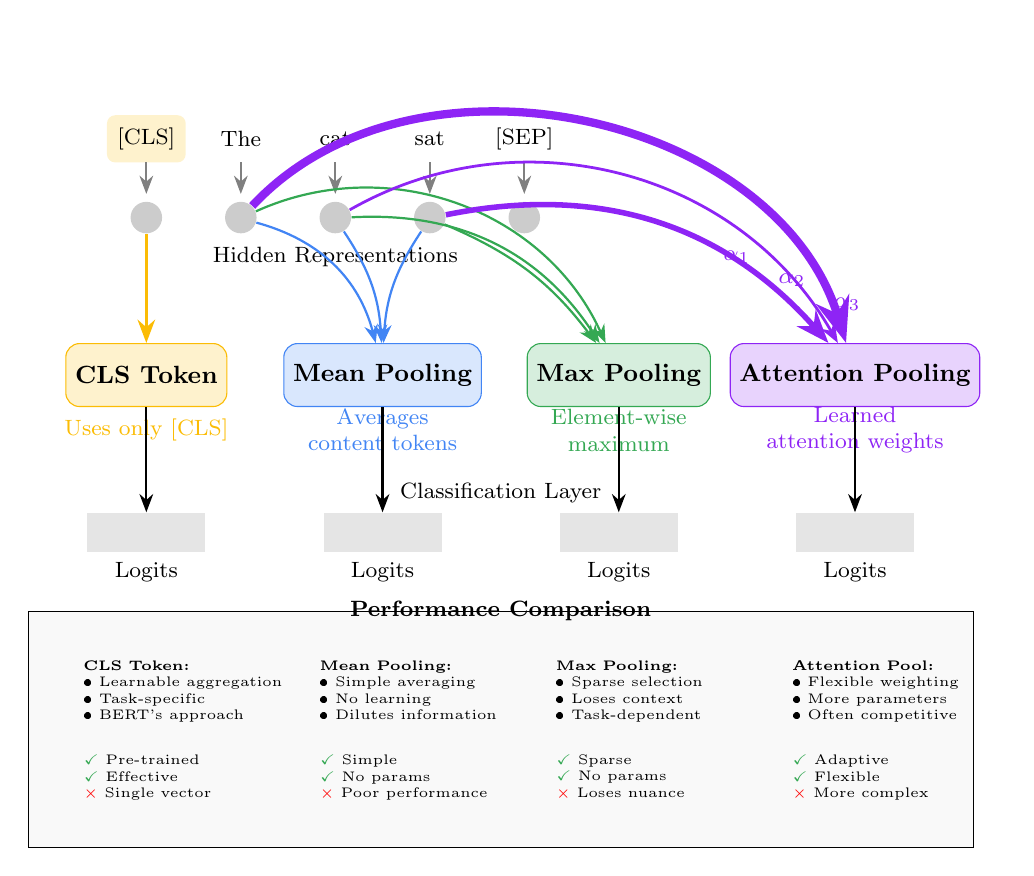
\begin{tikzpicture}[
    token/.style={rectangle, rounded corners=3pt, minimum width=1cm, minimum height=0.6cm, font=\footnotesize},
    hidden/.style={circle, fill=black!20, minimum size=0.4cm},
    arrow/.style={-{Stealth}, thick},
    pooling/.style={rectangle, rounded corners=5pt, minimum width=2cm, minimum height=0.8cm, font=\small\bfseries},
    label/.style={font=\footnotesize}
]

% === SPACING AND ALIGNMENT DOCUMENTATION ===
% Title: y=8.5, centered at x=6
% Input tokens: y=7, spaced 1.2cm apart horizontally
% Hidden representations: y=6, aligned with tokens above
% Pooling methods: y=4, evenly distributed at x=0,3,6,9
% Method descriptions: y=3.3
% Classification layer: y=2
% Comparison table: y=0 to -1.5, divided into 4 columns


% Input tokens (shared across all methods)
\node[token, fill=clsorange!20] (cls) at (0, 7) {[CLS]};
\node[token, fill=white] (t1) at (1.2, 7) {The};
\node[token, fill=white] (t2) at (2.4, 7) {cat};
\node[token, fill=white] (t3) at (3.6, 7) {sat};
\node[token, fill=white] (sep) at (4.8, 7) {[SEP]};

% Hidden representations
\node[hidden] (h0) at (0, 6) {};
\node[hidden] (h1) at (1.2, 6) {};
\node[hidden] (h2) at (2.4, 6) {};
\node[hidden] (h3) at (3.6, 6) {};
\node[hidden] (h4) at (4.8, 6) {};

% Arrows from tokens to hidden states
\foreach \i in {0,1,2,3,4} {
    \draw[arrow, gray] (\i*1.2, 6.7) -- (\i*1.2, 6.3);
}

\node[label] at (2.4, 5.5) {Hidden Representations};

% Method 1: CLS Token
\node[pooling, fill=clsorange!20, draw=clsorange] (cls_method) at (0, 4) {CLS Token};
\draw[arrow, clsorange, very thick] (h0) -- (cls_method);
\node[label, clsorange] at (0, 3.3) {Uses only [CLS]};

% Method 2: Mean Pooling  
\node[pooling, fill=bertblue!20, draw=bertblue] (mean_method) at (3, 4) {Mean Pooling};
\draw[arrow, bertblue] (h1) to[bend left=30] (mean_method);
\draw[arrow, bertblue] (h2) to[bend left=15] (mean_method);
\draw[arrow, bertblue] (h3) to[bend right=15] (mean_method);
\node[label, bertblue, align=center] at (3, 3.3) {Averages\\content tokens};

% Method 3: Max Pooling
\node[pooling, fill=gptgreen!20, draw=gptgreen] (max_method) at (6, 4) {Max Pooling};
\draw[arrow, gptgreen] (h1) to[bend left=45] (max_method);
\draw[arrow, gptgreen] (h2) to[bend left=30] (max_method);
\draw[arrow, gptgreen] (h3) to[bend left=15] (max_method);
\node[label, gptgreen, align=center] at (6, 3.3) {Element-wise\\maximum};

% Method 4: Attention Pooling
\node[pooling, fill=poolviolet!20, draw=poolviolet] (att_method) at (9, 4) {Attention Pooling};

% Attention weights visualization
\node[label, poolviolet] at (7.5, 5.5) {$\alpha_1$};
\node[label, poolviolet] at (8.2, 5.2) {$\alpha_2$};
\node[label, poolviolet] at (8.9, 4.9) {$\alpha_3$};

\draw[arrow, poolviolet, line width=3pt] (h1) to[bend left=60] (att_method);
\draw[arrow, poolviolet, line width=1pt] (h2) to[bend left=45] (att_method);
\draw[arrow, poolviolet, line width=2pt] (h3) to[bend left=30] (att_method);

\node[label, poolviolet, align=center] at (9, 3.3) {Learned\\attention weights};

% Classification outputs
\node[label] at (4.5, 2.5) {Classification Layer};
\foreach \method/\x in {cls_method/0, mean_method/3, max_method/6, att_method/9} {
    \node[rectangle, fill=gray!20, minimum width=1.5cm, minimum height=0.5cm] (out\x) at (\x, 2) {};
    \draw[arrow] (\method) -- (out\x);
    \node[label] at (\x, 1.5) {Logits};
}

% Comparison table - properly aligned in 4 columns
\node[rectangle, draw=black, fill=gray!5, minimum width=12cm, minimum height=3cm] (table) at (4.5, -0.5) {};
\node[font=\footnotesize\bfseries] at (4.5, 1) {Performance Comparison};

% Column headers with consistent positioning - using smaller font
\begin{scope}[every node/.style={font=\tiny, align=left, anchor=north, text width=2.6cm}]
    \node at (0.5, 0.5) {\textbf{CLS Token:}\\• Learnable aggregation\\• Task-specific\\• BERT's approach};
    \node at (3.5, 0.5) {\textbf{Mean Pooling:}\\• Simple averaging\\• No learning\\• Dilutes information};
    \node at (6.5, 0.5) {\textbf{Max Pooling:}\\• Sparse selection\\• Loses context\\• Task-dependent};
    \node at (9.5, 0.5) {\textbf{Attention Pool:}\\• Flexible weighting\\• More parameters\\• Often competitive};
\end{scope}

% Pros and Cons - aligned below headers - using smaller font
\begin{scope}[every node/.style={font=\tiny, align=left, anchor=north, text width=2.6cm}]
    \node at (0.5, -0.7) {\textcolor{gptgreen}{$\checkmark$} Pre-trained\\\textcolor{gptgreen}{$\checkmark$} Effective\\\textcolor{red}{$\times$} Single vector};
    \node at (3.5, -0.7) {\textcolor{gptgreen}{$\checkmark$} Simple\\\textcolor{gptgreen}{$\checkmark$} No params\\\textcolor{red}{$\times$} Poor performance};
    \node at (6.5, -0.7) {\textcolor{gptgreen}{$\checkmark$} Sparse\\\textcolor{gptgreen}{$\checkmark$} No params\\\textcolor{red}{$\times$} Loses nuance};
    \node at (9.5, -0.7) {\textcolor{gptgreen}{$\checkmark$} Adaptive\\\textcolor{gptgreen}{$\checkmark$} Flexible\\\textcolor{red}{$\times$} More complex};
\end{scope};

\end{tikzpicture}
\end{document}